% 2012_anhui_liberal_q19_fig1: cuboid, oblique top face D-C-B-A
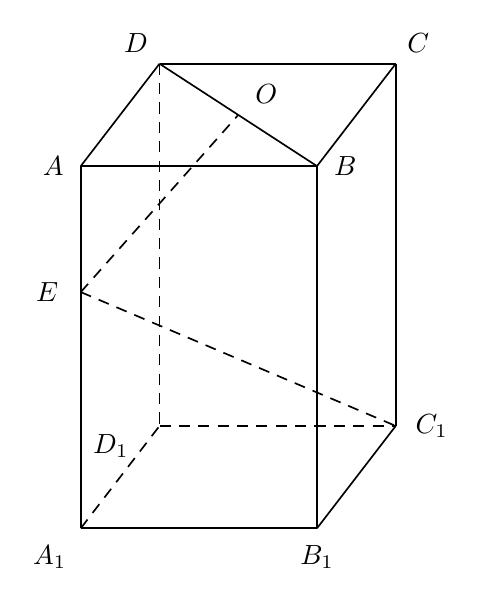
\begin{tikzpicture}[x=1cm,y=1cm,font=\normalsize,
  solid edge/.style={solid,line width=.6pt},
  hidden edge/.style={dashed,line width=.6pt,dash pattern=on 4pt off 3pt},
  geom label/.style={font=\normalsize,inner sep=2pt}]
\coordinate (D) at (1.2,5.2);
\coordinate (C) at (4.2,5.2);
\coordinate (B) at (3.2,3.9);
\coordinate (A) at (0.2,3.9);
\coordinate (D1) at (1.2,0.6);
\coordinate (C1) at (4.2,0.6);
\coordinate (B1) at (3.2,-0.7);
\coordinate (A1) at (0.2,-0.7);
\coordinate (O) at (2.2,4.55);
\coordinate (E) at (0.2,2.3);
% top face
\draw[solid edge] (D) -- (C);
\draw[solid edge] (A) -- (B);
\draw[solid edge] (D) -- (A);
\draw[solid edge] (D) -- (B);
\draw[solid edge] (C) -- (B);
% verticals / front
\draw[solid edge] (A) -- (A1);
\draw[solid edge] (B) -- (B1);
\draw[solid edge] (C) -- (C1);
\draw[solid edge] (A1) -- (B1);
\draw[solid edge] (B1) -- (C1);
% dashed interior / back
\draw[hidden edge] (D) -- (D1);
\draw[hidden edge] (D1) -- (C1);
\draw[hidden edge] (A1) -- (D1);
\draw[hidden edge] (E) -- (O);
\draw[hidden edge] (E) -- (C1);
\node[geom label,above left,xshift=-2pt,yshift=2pt] at (D) {$D$};
\node[geom label,above right,xshift=2pt,yshift=2pt] at (C) {$C$};
\node[geom label,left,xshift=-4pt] at (A) {$A$};
\node[geom label,right,xshift=4pt] at (B) {$B$};
\node[geom label,above right,xshift=4pt,yshift=2pt] at (O) {$O$};
\node[geom label,left,xshift=-6pt] at (E) {$E$};
\node[geom label,right,xshift=5pt] at (C1) {$C_{1}$};
\node[geom label,below,yshift=-4pt] at (B1) {$B_{1}$};
\node[geom label,below left,xshift=-3pt,yshift=-4pt] at (A1) {$A_{1}$};
\node[geom label,below left,xshift=-9pt,yshift=-1pt] at (D1) {$D_{1}$};
\end{tikzpicture}
